% !TEX program = xelatex

% Template file for an a0 landscape poster.
% Written by Graeme, 2001-03 based on Norman's original microlensing
% poster.
%
% See discussion and documentation at
% <http://www.astro.gla.ac.uk/users/norman/docs/posters/> 
%
% $Id: poster-template-landscape.tex,v 1.2 2002/12/03 11:25:46 norman Exp $


% Default mode is landscape, which is what we want, however dvips and
% a0poster do not quite do the right thing, so we end up with text in
% landscape style (wide and short) down a portrait page (narrow and
% long). Printing this onto the a0 printer chops the right hand edge.
% However, 'psnup' can save the day, reorienting the text so that the
% poster prints lengthways down an a0 portrait bounding box.
%
% 'psnup -w85cm -h119cm -f poster_from_dvips.ps poster_in_landscape.ps'

\documentclass[a0]{a0poster}
% You might find the 'draft' option to a0 poster useful if you have
% lots of graphics, because they can take some time to process and
% display. (\documentclass[a0,draft]{a0poster})
\input defs
\pagestyle{empty}
\setcounter{secnumdepth}{0}
\renewcommand{\familydefault}{\sfdefault}
\newcommand{\QED}{~~\rule[-1pt]{8pt}{8pt}}\def\qed{\QED}

\renewcommand{\reals}{{\mbox{\bf R}}}

% The textpos package is necessary to position textblocks at arbitary 
% places on the page.
\usepackage[absolute]{textpos}

\usepackage{fleqn,psfrag,wrapfig,tikz}

\usepackage[papersize={38in,28in}]{geometry}

% Graphics to include graphics. Times is nice on posters, but you
% might want to switch it off and go for CMR fonts.
\usepackage{graphics}


% we are running pdflatex, so convert .eps files to .pdf
%\usepackage[pdftex]{graphicx}
%\usepackage{epstopdf}

% These colours are tried and tested for titles and headers. Don't
% over use color!
\usepackage{color}
\definecolor{Red}{rgb}{0.9,0.0,0.1}

\definecolor{bluegray}{rgb}{0.15,0.20,0.40}
\definecolor{bluegraylight}{rgb}{0.35,0.40,0.60}
\definecolor{gray}{rgb}{0.3,0.3,0.3}
\definecolor{lightgray}{rgb}{0.7,0.7,0.7}
\definecolor{darkblue}{rgb}{0.2,0.2,1.0}
\definecolor{darkgreen}{rgb}{0.0,0.5,0.3}

\renewcommand{\labelitemi}{\textcolor{bluegray}\textbullet}
\renewcommand{\labelitemii}{\textcolor{bluegray}{--}}

\setlength{\labelsep}{0.5em}


% see documentation for a0poster class for the size options here
\let\Textsize\normalsize
%\def\Head#1{\noindent\hbox to \hsize{\hfil{\LARGE\color{bluegray} #1}}\bigskip}
\def\Head#1{\noindent{\LARGE\color{bluegray} #1}\bigskip}
\def\LHead#1{\noindent{\LARGE\color{bluegray} #1}\bigskip}
\def\Subhead#1{\noindent{\large\color{bluegray} #1}\bigskip}
\def\Title#1{\noindent{\VeryHuge\color{Red} #1}}


% Set up the grid
%
% Note that [40mm,40mm] is the margin round the edge of the page --
% it is _not_ the grid size. That is always defined as 
% PAGE_WIDTH/HGRID and PAGE_HEIGHT/VGRID. In this case we use
% 23 x 12. This gives us three columns of width 7 boxes, with a gap of
% width 1 in between them. 12 vertical boxes is a good number to work
% with.
%
% Note however that texblocks can be positioned fractionally as well,
% so really any convenient grid size can be used.
%
\TPGrid[40mm,40mm]{23}{12}      % 3 cols of width 7, plus 2 gaps width 1

\parindent=0pt
\parskip=0.2\baselineskip

% Our package definitions
\usepackage{optidef}
\usepackage{pspicture}
\usepackage{psfrag}
\usepackage{mathrsfs}
\usepackage{graphicx}
\usepackage{amsmath}
\usepackage{amsfonts}
\usepackage[small,bf]{caption}
\usepackage[usenames,dvipsnames]{pstricks}
\usepackage{epsfig}
%\usepackage{pst-grad} % For gradients
%\usepackage{pst-plot} % For axes
%\usepackage[space]{grffile} % For spaces in paths
%\usepackage{etoolbox} % For spaces in paths
\makeatletter % For spaces in paths
\patchcmd\Gread@eps{\@inputcheck#1 }{\@inputcheck"#1"\relax}{}{}
\makeatother

\newcommand{\linop}{\mathscr{L}}
\newcommand{\idop}{\mathbb{I}}
\newcommand{\ip}[1]{\left\langle{#1}\right\rangle}
\newcommand{\haml}{\mathcal{H}}

\DeclareMathOperator{\tr}{tr}

\begin{document}

% Understanding textblocks is the key to being able to do a poster in
% LaTeX. In
%
%    \begin{textblock}{wid}(x,y)
%    ...
%    \end{textblock}
%
% the first argument gives the block width in units of the grid
% cells specified above in \TPGrid; the second gives the (x,y)
% position on the grid, with the y axis pointing down.

% You will have to do a lot of previewing to get everything in the 
% right place.

% This gives good title positioning for a portrait poster.
% Watch out for hyphenation in titles - LaTeX will do it
% but it looks awful.
\begin{textblock}{23}(0,0)
\Title{LEigOpt: Fast Eigenvalue Optimization for Spectral-Element PDEs}
\end{textblock}

\begin{textblock}{23}(0,0.6)
{
\LARGE
Guillermo Angeris and John Sholar
}

{
\Large
\color{bluegray}
\emph{EE364b: Convex Optimization II Class Project}
}
\end{textblock}


% Uni logo in the top right corner. A&A in the bottom left. Gives a
% good visual balance, but you may want to change this depending upon
% the graphics that are in your poster.
%\begin{textblock}{2}(0,10)
%Your logo here
%%\includegraphics{/usr/local/share/images/AandA.epsf}
%\end{textblock}

%\begin{textblock}{2}(21.2,0)
%Another logo here
%%\resizebox{2\TPHorizModule}{!}{\includegraphics{/usr/local/share/images/GUVIu/GUVIu.eps}}
%\end{textblock}


\begin{textblock}{7.0}(0,1.5)

\hrule\medskip
\Head{Introduction}\\
Eigenvalue optimization is a common task in many control problems, inverse design, and, recently, in inference problems on continuous spaces. For this project, we attempted a few methods for fast solutions for eigenvalue problems arising from spectral element discretizations of eigenvalue partial differential equations (PDEs).

\medskip
\hrule\medskip
\Head{Spectral Element Methods and Laplacians} \\
A \textit{spectral element method} (SEM) is a finite-element method for solving PDEs which makes use of high-degree polynomials to approximate functions on a compact domain. The idea is to construct a quadrature rule such that all polynomials of lesser degree have exact integrals when sampled at a particular set of points, and generate some basis polynomials of degree less than the maximum.

In general, the Laplacians of these SEM-discretized problems---while sparse---usually incur a large computational cost on modern optimization packages for even a modest number of points. This is because the matrix generated by the spectral elements method is essentially a block-diagonal matrix with small blocks, each of which overlap with the previous block by exactly one element (see Figure~\ref{fig:overlap}), so no completely trivial decomposition can be applied.

\begin{figure}
\begin{center}
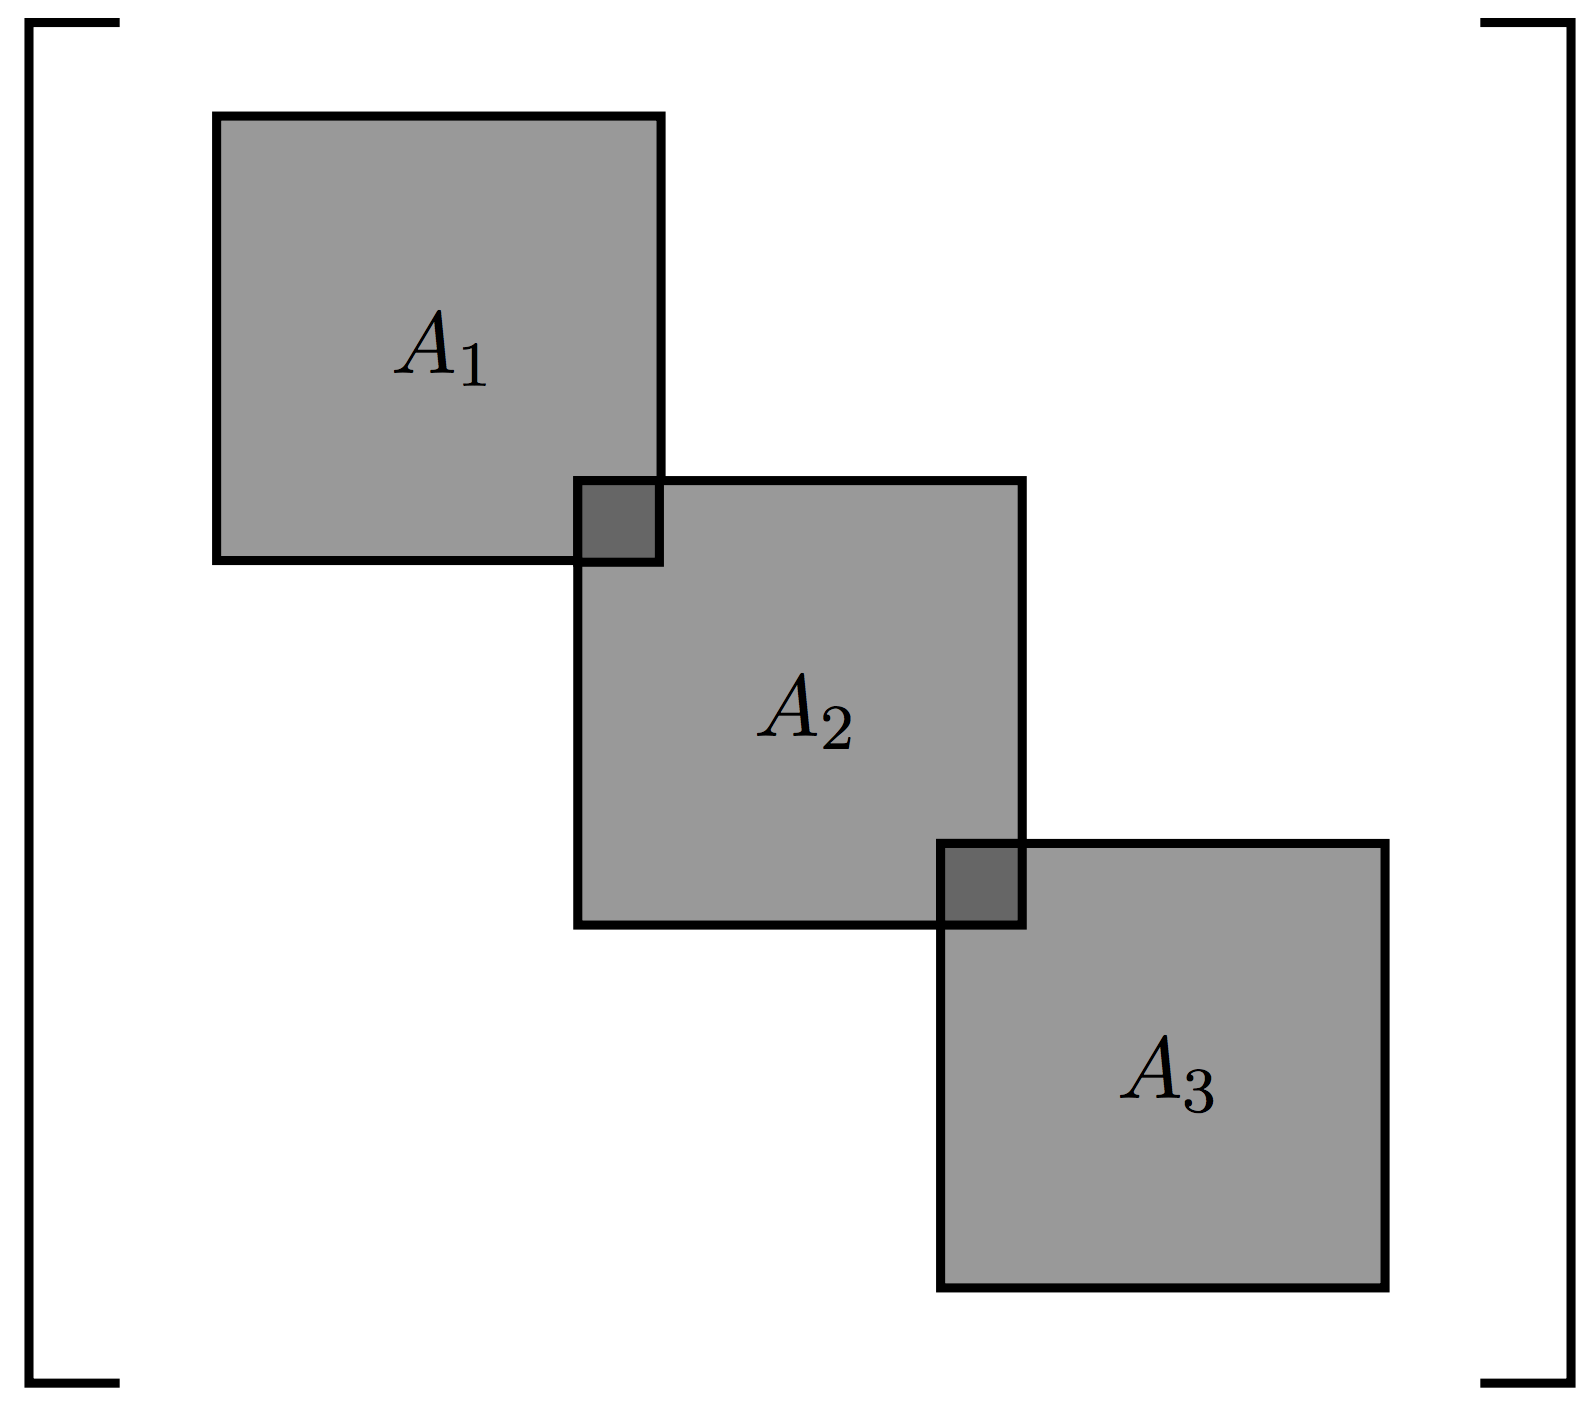
\includegraphics[width=.5\textwidth]{figures/overlap.png}
\caption{A simple example of the overlapping diagonal elements with three blocks. The darker box indicates a single overlapping element, e.g., $(A_1)_{nn} = (A_2)_{11}$ if $A_1 \in \reals^{n\times n}$.}
\label{fig:overlap}
\end{center}
\end{figure}
Our project takes advantage of the structure of these approximately-block-diagonal matrices for fast solutions of eigenvalue problems.

\medskip
\hrule\medskip
\Head{Problem}\\
Let $\linop: \reals^n \to \symm^m$ be affine and have the approximately-block-diagonal structure described in figure \ref{fig:overlap} and let $x \in \reals^n$, then the problem of interest can be written as the dual of a standard-form SDP,
\begin{maxi}
{x, t}{b^Tx + t}{}{\label{eq:optim}}
\addConstraint{\linop(x)}{\gek tI} 
\addConstraint{Cx}{=d}
\addConstraint{x}{\gek 0}.
\end{maxi}
The first inequality is with respect to the semidefinite cone, while the latter is with respect to the positive orthant.

\end{textblock}

\begin{textblock}{7.0}(8,1.5)

\hrule\medskip
\Head{Alternating Projections}\\
We can rewrite~(\ref{eq:optim}) as
\begin{mini*}
{x, t}{c^{T}x}{}{}
\addConstraint{\linop(x)}{=\sum_i E_i Z_i E_i^T} 
\addConstraint{Cx}{=d}
\addConstraint{x}{\gek 0}
\addConstraint{Z_i}{\gek 0,}{~ i\in\{1, 2, \dots, b\}},
\end{mini*}
where $E_{i} \in \reals^{n \times b}$ are selector matrices which project $Z_{i} \in \reals^{b \times b}$ into their appropriate position aligned with $\linop(x) - tI$ in $\reals^{n \times n}$. If $b \ll n$ projecting the $Z_i$ into the PSD cone is potentially much faster than projecting the complete matrix.

In order to construct the projections in question, we derive conditions for optimality as follows. From strong duality we have,
\[
    b^{T}x + d^{T}\eta - \tr(\Lambda A_{0}) = 0,
\]
while, from dual feasibility we have,
\[
    c_{i} + \tr(\Lambda A_{i}) + (C^T \eta)_{i} = \xi_{i}~~ \forall i,\hspace{2em}
    -E_{j}^{T} \Lambda E_{j} = \Sigma_{j} ~~ \forall j.
\]
Primal feasibility implies,
\[
    \linop(x) = \sum_{j} E_{j} Z_{j} E_{j}^{T},
    \hspace{2em}
    x \gek 0,
    \hspace{2em}
    Z_{j} \gek 0 ~~ \forall j,
    \hspace{2em}
    Cx = d,
\]
while dual feasibility implies,
\[
    \Sigma_{j} \gek 0 ~~ \forall j,
    \hspace{2em}
    \xi_{i} \geq 0 ~~ \forall i.
\]
These are all either affine spaces or convex cones, so we can find a point in the intersection of all sets via alternating projections. Since the affine projections can be computed and cached in the pre-solve, and projecting into PSD cones is simple for $Z_j, \Sigma_j \in \reals^{b\times b}$. As $b \ll n$, this formulation yields a speed up in computational time.

\medskip
\hrule\medskip
\Head{Optimizations}\\
Many of our projections involve projecting a variable $y$ onto $\{x~|~Cx = d\}$. One standard projection in this case is given by
\[
    \Pi_{\{x|Cx = d\}}(y) = C^{\dagger}d + (I -  C^{\dagger}C)y
\]
However, in the case that $C \in \reals^{k \times n}$, where $y \in \reals^{n}$, this can be computed much more efficiently, specifically by computing the QR factorization of $C^{T}$ and noting that given $QR = C^{T}$ we have 
\begin{align*}
    C^{\dagger}C &= C^{T}(CC^{T})^{-1}C\\
    &= QR(R^{T}Q^{T}QR)^{-1}R^{T}Q^{T}\\
    &= QQ^T
\end{align*}


\end{textblock}

\begin{textblock}{7.0}(16,1.5)

\hrule\medskip
\Head{Results}\\

To compare the efficiency of our methods to the standard SCS solver, we test the performance of both on an eigenvalue derivation problem, which can be formulated as a special case of~(\ref{eq:optim}).

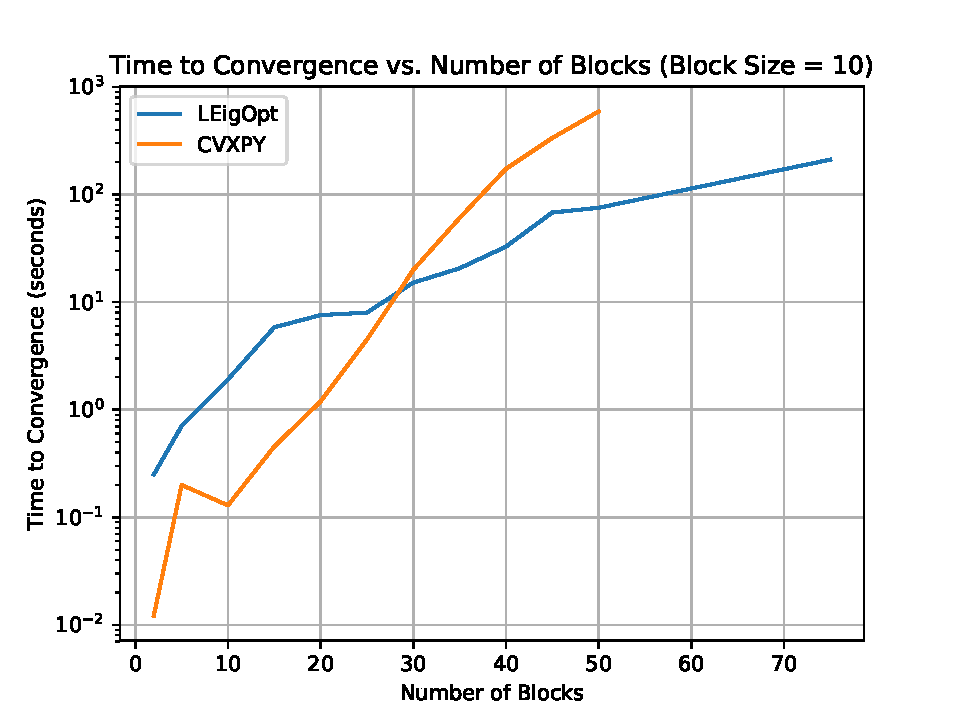
\includegraphics[width=.5\textwidth]{figures/fixed_block_size.pdf}
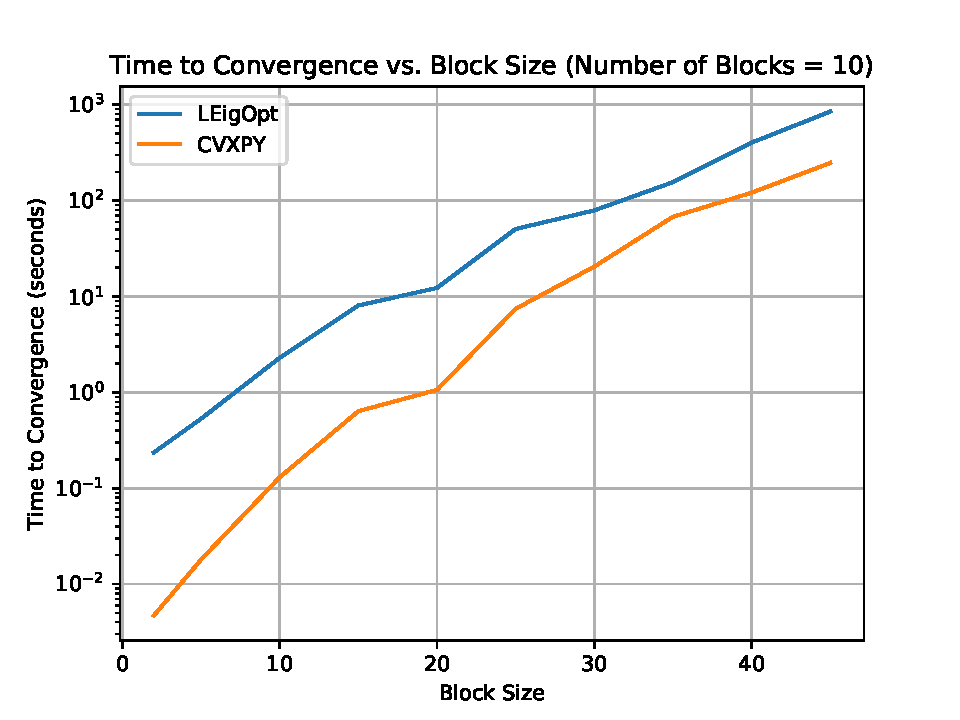
\includegraphics[width=.5\textwidth]{figures/fixed_num_blocks.pdf}
\begin{itemize}
\item Fixing the number of blocks $N$ to be 10 and varying $b$, SCS outperforms LEigOpt consistently, but the gap narrows from a factor of 100 ($b = 2$) to a factor of 3 ($b = 45$).
\item Fixing $b = 10$ and varying $N$, SCS initially outperforms LEigOpt, but is surpassed at around $N = 30$. As the block count increases, LEigOpt consistently outperforms SCS---more specifically, convergence times for LEigOpt grow roughly linearly, while those for SCS grow roughly quadratically, if not cubically. SCS did not finish at $N=75$.
\item It should also be noted that large portions of our solver are written in Python (interpreted, slow) on top of NumPy libraries, while the CVXPY SCS solver is written in C (compiled, fast).
\end{itemize}

\medskip
\hrule\medskip
\Head{Future Work: Interior-Point Methods}\\
For interior point methods, rewriting the problem using a barrier method is straightforward:
\begin{maxi*}
{x, t}{b^Tx + t + \mu\log \det (\linop(x)-tI)}{}{}
\addConstraint{Cx}{=d}
\addConstraint{x}{\gek 0}.
\end{maxi*}

The $\linop(x)$ matrix, with the given sparsity pattern, can be forced to have block-diagonal structure on the top-left block, with narrow bands on the bottom and rights sides, via some permutation matrix $P$, with
\[
\hat \linop(x) = P\linop(x)P^T.
\]
This matrix, $\hat \linop(x)$ has a simple Cholesky decomposition, which can be exploited for fast computation of the barrier function and its first and second derivatives for use with a Newton or Newton-like method.


\end{textblock}


\end{document}
